\documentclass[tikz, border=10pt]{standalone}
\usepackage{tikz}
\usetikzlibrary{shapes, arrows.meta, positioning}

\definecolor{bluePolimi}{RGB}{34, 41, 53}
\definecolor{lightBluePolimi}{RGB}{91, 122, 172}
\definecolor{greenPolimi}{RGB}{0, 110, 0}
\definecolor{redPolimi}{RGB}{180, 0, 0}
\definecolor{yellowPolimi}{RGB}{255, 204, 0}

\begin{document}
    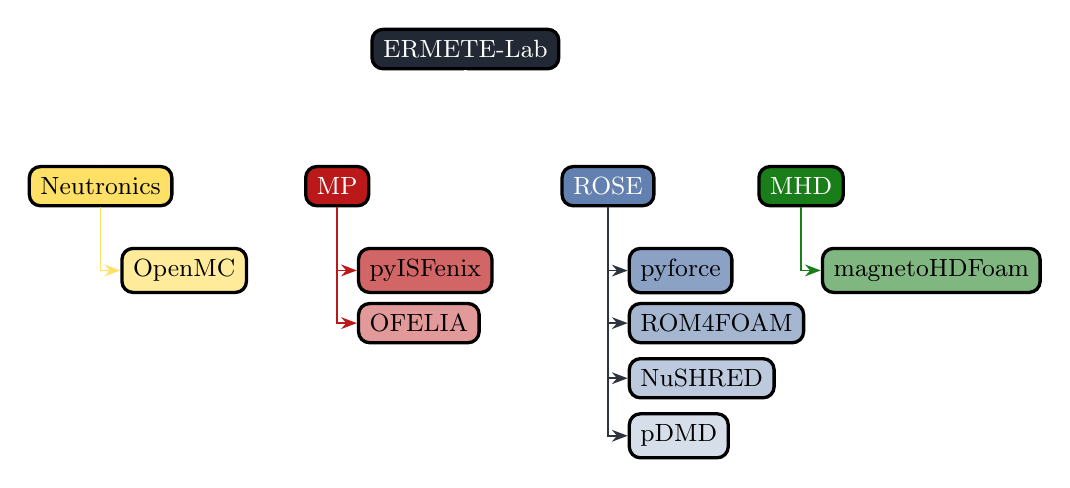
\begin{tikzpicture}[>=Stealth, every node/.style={font=\small}, line width=1.2pt]
        
        \tikzstyle{org} = [rectangle, draw, fill=bluePolimi, text centered, rounded corners, text=white, inner sep=4pt]
        \tikzstyle{arrow} = [->, >=Stealth]
        
        % Nodo Principale
        \node (superorg) [org] {ERMETE-Lab};
        
        % --- Categorie Principali ---
        % Neutronics
        \node (neutronics) [org, below left=1.2cm and 2.5cm of superorg, fill=yellowPolimi!60, text=black] {Neutronics};
        % MP
        \node (mp) [org, below left=1.2cm and 0.cm of superorg, fill=redPolimi!90] {MP};
        % ROSE
        \node (rose) [org, below right=1.2cm and 0.cm of superorg, fill=lightBluePolimi!95] {ROSE};
        % MHD
        \node (mhd) [org, below right=1.2cm and 2.5cm of superorg, fill=greenPolimi!90] {MHD};
        
        % --- Sotto-elementi (spostati a destra rispetto al centro del genitore) ---
        % Neutronics
        \node (openmc) [org, below right=0.5cm and 0.25cm of neutronics.south, fill=yellowPolimi!40, text=black] {OpenMC};

        % MP
        \node (isf)    [org, below right=0.5cm and 0.25cm of mp.south, fill=redPolimi!60, text=black] {pyISFenix};
        \node (ofelia) [org, below right=1.2cm and 0.25cm of mp.south, fill=redPolimi!40, text=black] {OFELIA};

        % ROSE
        \node (pyforce)  [org, below right=0.5cm and 0.25cm of rose.south, fill=lightBluePolimi!70, text=black] {pyforce};
        \node (rom4foam) [org, below right=1.2cm and 0.25cm of rose.south, fill=lightBluePolimi!55, text=black] {ROM4FOAM};
        \node (nushred)  [org, below right=1.9cm and 0.25cm of rose.south, fill=lightBluePolimi!40, text=black] {NuSHRED};
        \node (pdmd)     [org, below right=2.6cm and 0.25cm of rose.south, fill=lightBluePolimi!25, text=black] {pDMD};
        
        % MHD
        \node (loverso) [org, below right=0.5cm and 0.25cm of mhd.south, fill=greenPolimi!50, text=black] {magnetoHDFoam};
        
        % --- Frecce Superiori (Tuo stile originale) ---
        \draw [arrow, white] (superorg.south) |- (0,-0.7) -| (neutronics.north);
        \draw [arrow, white] (superorg.south) |- (0,-0.7) -| (mp.north);
        \draw [arrow, white] (superorg.south) |- (0,-0.7) -| (rose.north);
        \draw [arrow, white] (superorg.south) |- (0,-0.7) -| (mhd.north);

        % --- Frecce Inferiori (Tuo stile originale: escono da south ed entrano in west) ---
        \draw [arrow, line width=0.6pt, yellowPolimi!60] (neutronics.south) |- (openmc.west);

        \draw [arrow, line width=0.6pt, redPolimi!90] (mp.south) |- (isf.west);      
        \draw [arrow, line width=0.6pt, redPolimi!90] (mp.south) |- (ofelia.west);   

        \draw [arrow, line width=0.6pt, bluePolimi!95] (rose.south) |- (pyforce.west);        
        \draw [arrow, line width=0.6pt, bluePolimi!95] (rose.south) |- (rom4foam.west);       
        \draw [arrow, line width=0.6pt, bluePolimi!95] (rose.south) |- (nushred.west);        
        \draw [arrow, line width=0.6pt, bluePolimi!95] (rose.south) |- (pdmd.west);       
        
        \draw [arrow, line width=0.6pt, greenPolimi!90] (mhd.south) |- (loverso.west);     
        
    \end{tikzpicture}
\end{document}